\documentclass[11pt]{article}
\usepackage[utf8]{inputenc}
\usepackage[margin=1in]{geometry}
\usepackage{float}
\usepackage{graphicx}
\usepackage{hyperref}
\usepackage{bookmark}
\usepackage[backend=biber, style=alphabetic, sorting=ynt]{biblatex}
 
\addbibresource{main.bib}
\title{Mini-Assignment: CS3423 - Compilers - II}
\author{Vishwak Srinivasan\\
\texttt{CS15BTECH11043}
\and
Harsh Agarwal\\
\texttt{CS15BTECH11019}
}
\date{}

\begin{document}

\maketitle

\section{Introduction}
The current widespread interest in protecting software from piracy, tampering, and reverse engineering has been brought to bear for several reasons. Some of these include that revenue derived from proprietary software sales is vital to many software vendors’ survival, more vendors distribute software in forms that attackers can easily manipulate. This field is inherently practical, and thus of industrial relevance: indeed, protecting a piece of software against tampering, malicious modifications or reverse-engineering is a very difficult task.
\(\newline\)

A defense against tampering is what is known as \textbf{tamper-proofing}, so that unauthorized modifications to software (for example to remove a watermark) will result in non-functional code. Tamper-resistant software typically uses built-in integrity checks to detect code tampering by guarding the code being executed, or by checking that the flow of control through the program is the expected one.
\(\newline\)

\textbf{Anti-Debugging} techniques are ways for a program to detect if it is running under the control of a debugger or a dissembler. 
A debugger places an important role while reverse engineering a program. When a program is being debugged, the operating system needs to modify the debugger's environment for the debugging to start (however there are debuggers which can bypass this, for example: \texttt{Obsidian debugger}). One obvious anti-debugging technique can be to check the state of the environment but we explain below how such checks can be easily circumvented by the attacker. 
\(\newline\)

Although these methods may not provide as much resistance in due course of time, these methods could however increase the computational costs in breaking the existing barriers and enabling reverse engineering.

\section{Code Tamper-Proofing: a brief overview}
There are many situations where we would like to stop anyone from executing our program if it has been altered in any way.

\begin{figure}[H]
    \centering
    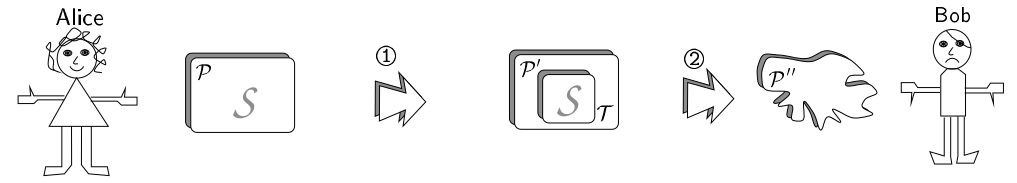
\includegraphics[width=0.75\linewidth]{tampering.png}
    \label{tampering-pic}
    \caption{Alice protects a secret \(\mathcal{S}\) by adding tamper-proofing code \(\mathcal{T}\) that makes the program fail if \(\mathcal{S}\) has been tampered with. Adapted from \emph{Watermarking, Tamper-Proofing, and Obfuscation - Tools for Software Protection} by Collberg et al \cite{Collberg:2002:WTO:636196.636198}}
\end{figure}
To prevent such tampering attacks we can add tamper-proofing code to our program. This code should be ideally able to achieve the following objectives:
\begin{itemize}
    \item \underline{detect} if the program has been altered
    \item make the program \underline{fail} if evidence of such alteration has been discovered.
\end{itemize}
In the above example: this tamper-proofing code should be ideally able to detect if Bob has tampered with \(\mathcal{S}\) in the program \(\mathcal{P}\), and if so, the code \(\mathcal{T}\) transforms \(\mathcal{P}\) to \(\mathcal{P}''\), which would fail.
\(\newline\)

Intuitively, it can be seen that this code tamper-proofing can be done in two simple ways:
\begin{enumerate}
    \item Perform a check on the executable (possibly fake) to see if it is the same as the original. we could always make use a check-sum to check the validity of the program. Popular and speedy check-sum hash-producers include MD5. \cite{Rivest:1992:MMA:RFC1321}
    \item Perform intermediate result value checking by comparing it with the intermediate results of the original. This notion of intermediate value checking is key in program analysis and verification. \cite{DBLP:conf/icalp/Blum93, DBLP:conf/fsttcs/Blum91}
\end{enumerate}

\section{Existing Methods in Tamper-Proofing}
Collberg et al \cite{DBLP:conf/popl/CollbergT99} have provided methods to ensure tamper-proofing in software watermarks. Based on this work and other techniques, Collberg, Myles and Huntwork were able to develop \textit{SANDMARK} \cite{DBLP:journals/ieeesp/CollbergMH03}, a tool for software protection research. This work has been left dormant for a while. Latest work in Code Tamper-proofing by Junod et al \cite{DBLP:conf/icse/JunodRWM15} have implemented Obfuscator-LLVM (\texttt{ollvm}) which has been integrated in the LLVM Suite.

\section{Code Tamper-Proofing in LLVM IR}
Work by Junod et al intuitively suggest the usage of two routines \texttt{check()} and \texttt{respond()}. Just as how it seems, \texttt{check()} is responsible to detect a modification, whereas \texttt{respond()} is responsible for providing an action in the advent of such modification made.

In \texttt{ollvm} as the authors have suggested, a tamper-proofing mechanism is available although it is integrated with a code-flattening module. This enables various \texttt{check()} to be inserted into the code. The result of the \texttt{check()} routine is responsible for the behaviour of the previously flattened code. 

\subsection{Implementation of \texttt{check()}}
The \texttt{check()} routine is implemented as the computation of a 32 - bit Cyclic Redundancy Check (CRC). At least 1 \texttt{check()} routine is placed at every basic block, and the location of the \texttt{check()} routine within the basic block is randomly chosen. The authors of \texttt{ollvm} mention that the return values of the \texttt{check()} routine manage the basic block routing variable. The routing is also statically dependent on a variable \(s\) where \(s = \rho \oplus d_{1} \oplus d_{2} \oplus \ldots \oplus d_{n}\) where \(\rho\) is a value leading to the next basic block and \(d_{i}\) is the result of the \(i^{th}\) \texttt{check()} routine in that basic block.

\subsection{\texttt{respond()}}
The invalid check-sum value drives the program in an infinite loop, hence corrupting the program.

\section{Ideas worth discovering}
\subsection{Why have multiple \texttt{check()} routines in one basic block?}
Work by Junod et al \cite{DBLP:conf/icse/JunodRWM15} have considered adding multiple \texttt{check()} routines in one basic block. But why are multiple \texttt{check()} routines required? If we are able to identify the ``secretive" part of that basic block, we could add just one \texttt{check()} routine there. Note that every \texttt{check()} routine incurs some overhead.

\subsection{Other methods for \texttt{check()}}
The authors of \texttt{ollvm} have considered CRC-32 for every \texttt{check()} routine. Note that CRC-32 is not resistant to intentional modifications to data. This is because of their convenient mathematical properties. 

We could always consider the implementation of other check-sum based algorithms. In fact, it would be nice to see an internal implementation of popular algorithms like MD5 or SHA-1\cite{Eastlake:2001:USH:RFC3174} which are hash-based algorithms as opposed to CRC.

\section{Anti Debugging Techniques}
\subsection{Popular Anti-Debugging Methods in Windows \footnote{\href{https://www.apriorit.com/dev-blog/367-anti-reverse-engineering-protection-techniques-to-use-before-releasing-software}{Anti-Reverse Engineering Protection Techniques}}}
Windows has many built in functions for checking whether a program is running under a debugger or not. Some popular ones are listed below. Interestingly we did not find much built-in support for anti-debugging support in Linux. Adding anti-debugging support in Linux can be  a good project to work upon.
\begin{itemize}
    \item{\textbf{Checking Anti-Debugging Flags before program execution : }\\
    Windows Operating System provides many flags in its PEB  (Process Environment Block) that can be used for testing whether a process is being run in debugger mode. \texttt{BeingDebugged}, \texttt{NtGlobalFlag}, \texttt{Heap Flags and ForceFlags} in the process heap are some flags that can be checked for checking whether a program is being debugged or dissembled by another process.
    \begin{itemize}
        \item {\textbf{Where to check for the flags? Thread Local Storage Callbacks}\\
        One important point to note is that checking these debugging flags in the main function is not the best idea because that's where the attacker usually starts to reverse-engineer. In Windows, Thread Local Storage is used to initialize thread-specific data before the main thread runs. Since every process has at least one thread, the check for such flags should be in 
        the TLS callback array which are executed whenever a thread is created or destroyed (including the thread created by Windows to attach the debugger to the process). Thus checking for the debugger flags should be done in the \textbf{TLS Callback}.
        }
        \item{\textbf{How to bypass?}\\
        These checks can easily be circumvented by an attacker by setting these flags to 0 before the anti-debugging check is done. The attacker can insert a breakpoint on the first byte of the first THS callback, instead at the host entrypoint to gain control before any code is run.}
    \end{itemize}
\textit{Scope for Improvement/Idea}:\\We could come up with innovative ways using \textbf{Code Obfuscation} \& \textbf{Code Restructuring} to make frequent calls to such checkers so that it is tough for the attacker to analyze where the checks are being made.
    }

    \item{\textbf{Using \texttt{NtQueryInformationProcess} :}\\ \texttt{NtQueryInformationProcess} is a function which retrieves information about a process. Using this information we can analyze and detect whether an attacker is debugging the code or not.

    \begin{itemize}
        \item{\texttt{ProcessInformationClass : }\\ By analyzing the value \texttt{ProcessInformationClass} returned by \\ \texttt{NtQueryInformationProcess} we can tell whether a process is being debugged by another parallel process. }
        \item{\texttt{ProcessDebugObjectHandle : }\\ For debugging purposes a debug object is created. Using \texttt{NtQueryInformationProcess}, we can detect whether this object exists or not.}
        \item{\texttt{ProcessBasicInformation : }\\ Using \texttt{ProcessBasicInformation} flag, the process's \texttt{PROCESS\_BASIC\_INFORMATION} is returned. From this structure we can get the \texttt{InheritedFromUniqueProcessId} field and compare the name of the parent process with the names of some popular debuggers. If there is a match we can tell that debugging is currently going on.}
        \item{\textbf{How to bypass?}\\ One major drawback of using \texttt{NtQueryInformationProcess} is that the attacker can easily change these values before any of the above debugging checks are called to prevent the check from failing.}
    \end{itemize}
    }
    \item{\textbf{Software Breakpoints}\\Reverse Engineering a program without using breakpoints is very hard. Hence popular anti-debugging tactics include detecting the presence of breakpoints in the program.
    Windows inserts an \texttt{int 3h} instruction to denote a break-point. Whenever this instruction is encountered the OS interrupts the program execution and the control is transferred to the debugger. Hence a possible anti-debugging method can be to search for such breakpoints in a program by calculating the check-sum of the function.}

    \item{\textbf{Hardware Breakpoints}\\There are certain debug registers provided by the x86 architecture that are used by developers to debug code. But they can only be used when the program is running in \textbf{real mode or safe mode with privilege level 0}. For production ready software these registers are never used. Therefore if at any instance of the program execution we find a non null value in these registers we can say that the program is being run in the debug mode.}
    
    \begin{itemize}
            \item{\textbf{How to bypass?}\\ Before the check for nullity of the registers is made, the attacker can reset these registers and restore them back again once the check is completed.}
    \end{itemize}

    \item{\textbf{SEH (Structured Exception Handling)}\\SEH is a mechanism provided by the operating system to an application allowing it to receive notifications about exceptions. During normal execution of a program if an exception occurs first the control goes to the SEH. The SEH returns certain \texttt{EXCEPTION\_DISPOSITION} which tells what the program should do the handle the exception. If none of the methods work SEH returns \texttt{ExceptionCollidedUnwind} disposition which essentially means calling the debugger present in the \texttt{REG\_SZ} file. If a program is being debugged , on encountering an \texttt{int 3h} instruction , the debugger will be called directly. Hence we can check whether the SEH was called to handle the exception.
    
     \begin{itemize}
            \item{\textbf{How to bypass?}\\ Before calling any SEH handler \texttt{ntdll!ExecuteHandler2} function is called. The attacker can insert a break-point at the call instruction to this function and analyze the consequent SEH handler flow of execution. Although bypassing SEH can be hard in real-life.}
    \end{itemize}
    
    \textit{Scope for Improvement/Idea:}\\To make the life harder for the attacker, we can include any calls to SEH handlers and using \textbf{Code Obfuscation} \& \textbf{Code Restructuring} can come up with innovative ways to place them.
    }
    \item{\texttt{NtSetInformationThread}\\For preventing debugging information from being transferred , the developer can set the field \texttt{ThreadHideFromDebugger} in the \texttt{\_ETHREAD } structure. This prevents a thread from sending any notifications about debug events like breakpoints and program completion.}
\end{itemize}
Apart from the above mentioned methods many other innovative anti-debugging ways exist. Some of them can be easily broken whereas some are hard to break.   
\textit{Scope for Improvement/Idea:} We can come up with ideas to combine the various anti-debugging methods to make the ultimate debugger that knows them all. 

\section{Conclusion of the Report}
Through this mini-assignment, we were made aware of the concepts of Code Tamper-proofing and Anti-debugging. In Code Tamper-proofing, we discussed some previous work in the area, and briefly mentioned about \texttt{ollvm} suite, which is the first complete LLVM suite to implement code protection techniques in one package. In Anti-debugging techniques, we surprisingly found that the Linux kernel doesn't have much current support for anti-debugging methods, whereas the NT kernel for Windows does. We also briefly mention some popular anti-debugging strategies that exist in Windows and mention ways how can these checks be circumvented by the attacker. Finally we also suggest some ideas that can be implemented to make such checks more robust and increase the difficulty for the attacker. 
% GG, robustness!!!!!!
% Generalization, ML, awesomeness
% Awesome stuff bro
% Compilers is dead, long live ML and optimization

\printbibliography
\end{document}
